\documentclass[a4paper,11pt]{article}
\usepackage[utf8]{inputenc}
\usepackage{tikz}
\usetikzlibrary{shapes}

\thispagestyle{empty} % no pagenumber. The form should be a stand alone macro... later.

\definecolor{SEPAOrange}{RGB}{254,213,161}
\definecolor{SEPABlindcolor}{RGB}{255,0,0}


\begin{document}


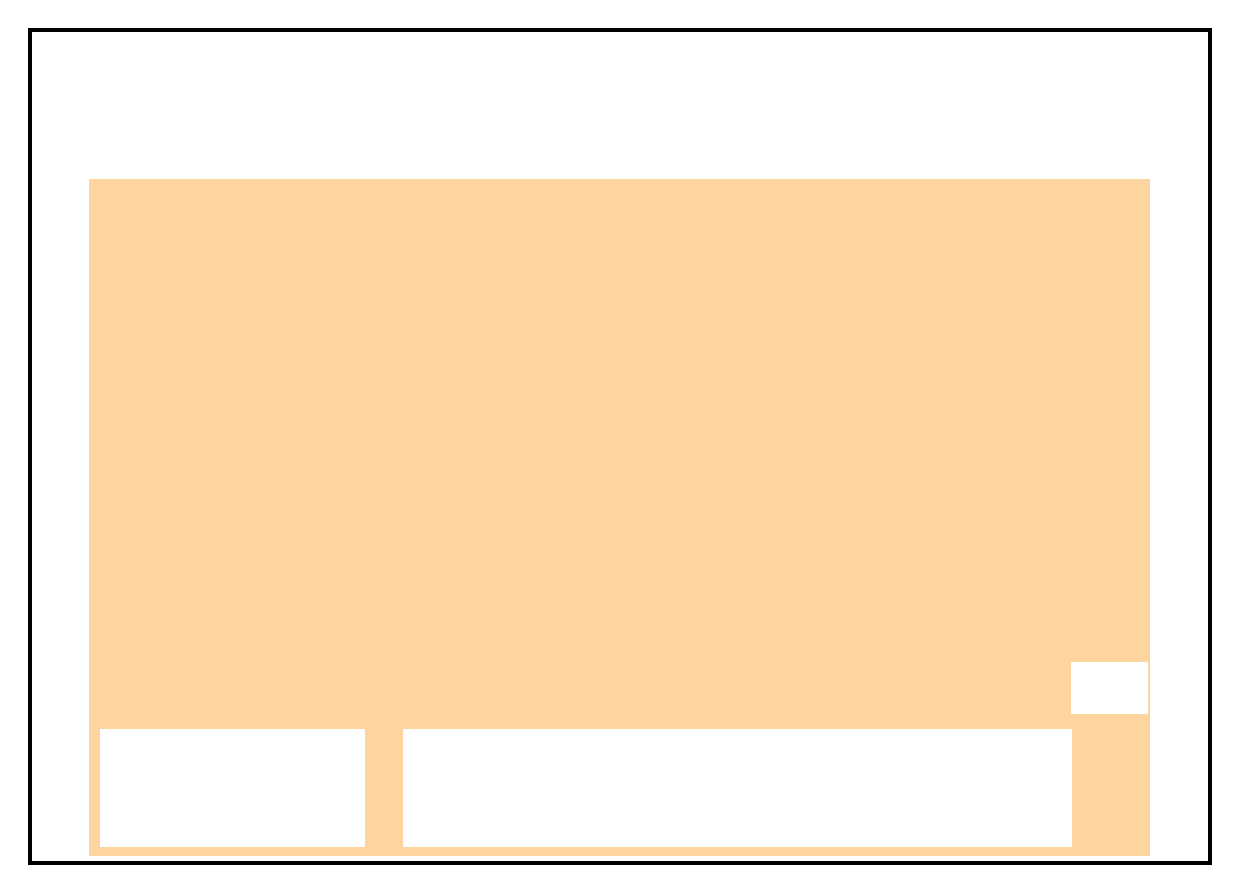
\begin{tikzpicture}[x=1 mm, y=-1mm]
\pgfmathsetmacro{\yw}{4.2333} % defined as 1/6 inch =>  1/6 * 25.4 mm = 4.2333 mm
%\pgfmathsetmacro{\xw}{4.2333} % defined as
\pgfmathsetmacro{\xs}{9} % x start (own definition)
\pgfmathsetmacro{\xe}{142} % x end (own definition)

\draw[draw=black,color=black, line width=0.5mm] (0,0) rectangle (149.86,105.83); %border
\filldraw[draw=black,color=SEPAOrange] (7.62, 4.5*\yw) rectangle (149.86-7.62,105.83-1); %orange background


\filldraw[draw=black,color=white] (149.86-17.59, 19* \yw) rectangle (\xe, 20.5*\yw); % counter
\filldraw[draw=black,color=white] (\xs, 21* \yw) rectangle (42.52, 24.5*\yw); % date
\filldraw[draw=black,color=white] (42.52+5, 21*\yw) rectangle (149.86-17.59, 24.5*\yw); % signature

%\draw[align=left] at (\yw,\yw) {SEPA-Überweisung};

\end{tikzpicture}
\end{document} 